\documentclass[aspectratio=169,9pt]{beamer}
\usetheme{default}
\usecolortheme{default}
\setbeamertemplate{navigation symbols}{}
\setbeamertemplate{footline}{}
\setbeamersize{text margin left=8mm,text margin right=8mm}
\usepackage[T1]{fontenc}
\usepackage{lmodern}
\usepackage{booktabs}
\usepackage{graphicx}
\usepackage{amsmath,amssymb}
\usepackage{xcolor}

\definecolor{StanfordRed}{RGB}{140,21,21}
\definecolor{NavyDark}{RGB}{15,41,66}
\definecolor{SlateBg}{RGB}{244,246,250}

\setbeamercolor{frametitle}{fg=NavyDark}
\setbeamertemplate{frametitle}{%
  \vspace{4pt}
  {\normalsize\bfseries\insertframetitle\par}
  {\scriptsize\color{StanfordRed}\insertframesubtitle\par}
  \vspace{2pt}\hrule height 0.6pt \vspace{3pt}
}

\begin{document}
\begin{frame}{Spectral weighting resists cloned judges on held-out benchmarks}{The gain is largest when a weak or anti-correlated judge is replicated. Clean ensembles still trail the strongest individual judge.}
\begin{columns}[T,totalwidth=\textwidth]
\begin{column}{0.51\textwidth}
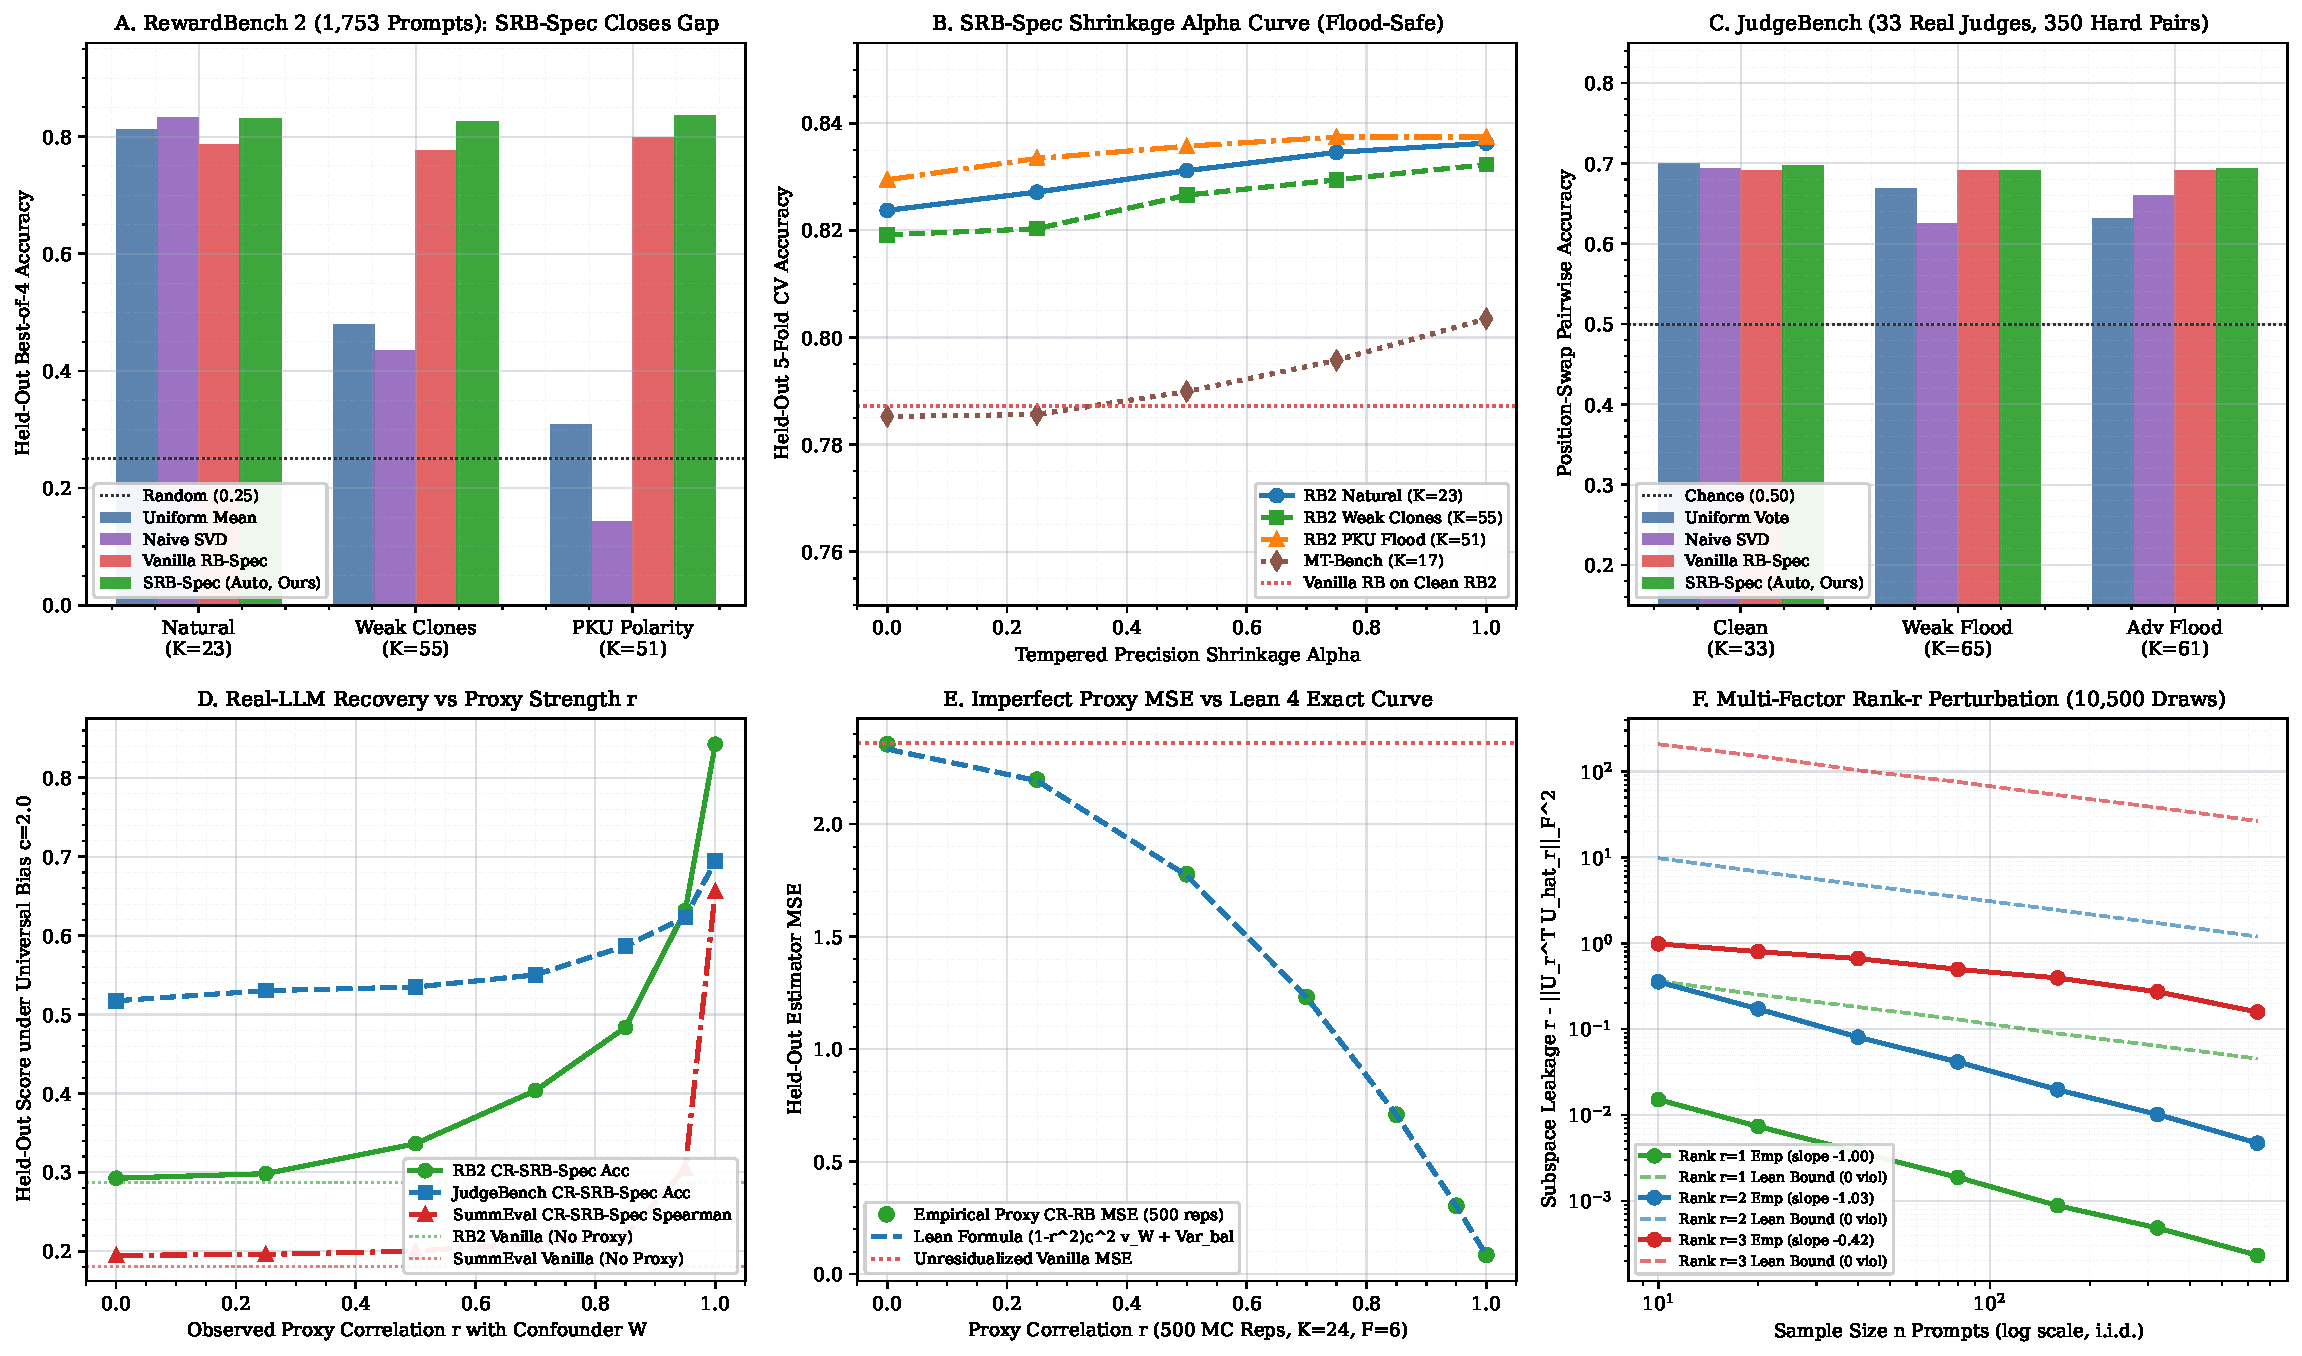
\includegraphics[width=\linewidth]{../../latex_paper/neurips/figures/exp15_srb_judgebench_proxies_and_multifactor_6panel.pdf}
\end{column}
\begin{column}{0.47\textwidth}
{\small\bfseries Five-fold held-out performance}\par\smallskip
{\scriptsize\setlength{\tabcolsep}{3pt}
\begin{tabular*}{\linewidth}{@{\extracolsep{\fill}}lrr@{}}
\toprule
Panel & Plain SVD & Adjusted\\
\midrule
RewardBench 2, 23 judges & .833 & .836\\
\quad +32 weak replicas & .435 & .832\\
\quad +28 anti-correlated replicas & .143 & .837\\
JudgeBench, 33 judges & .694 & .714\\
\quad +28 inverted replicas & .660 & .711\\
SummEval, mixed panel & .486 & .647\\
MT-Bench, 17 signals & .716 & .803\\
\bottomrule
\end{tabular*}}\par\medskip
{\scriptsize Adjusted scores use fixed shrinkage for RewardBench~2, SummEval and MT-Bench, and covariate adjustment on JudgeBench. SummEval reports pooled Spearman correlation. Other rows report accuracy. SVD denotes singular value decomposition.}\par\medskip
{\scriptsize With 20 human anchor articles, mean SummEval ensemble bias fell from $-1.104$ to $+0.007$ points and absolute agreement rose from .334 to .644.}
\end{column}
\end{columns}
\vfill
{\scriptsize\textbf{Scope.} RewardBench~2 includes 1,753 prompts, JudgeBench 350 pairs, SummEval 1,600 summaries from 100 articles, and MT-Bench 2,575 decisive ratings on 80 questions. The best individual judge reached .892 on RewardBench~2 and .754 on JudgeBench.}\par\smallskip
{\scriptsize\textbf{Formal and simulation results.} Lean~4 checks 66 theorems, including a residual-variance identity for an imperfect proxy and a conditional spectral bound. The bound held in all 10,500 sampled rank and sample-size trials.}
\end{frame}
\end{document}
